\renewcommand{\leveltopI}{-15cm + \leveltop}
\renewcommand{\leveltopII}{-15cm + \leveltopI}
\renewcommand{\leveltopIII}{-15cm + \leveltopII}
\renewcommand{\leveltopIIII}{-15cm + \leveltopIII}
\renewcommand{\leveltopIIIII}{-15cm + \leveltopIIII}
\renewcommand{\leveltopIIIIII}{-15cm + \leveltopIIIII}
\renewcommand{\leveltopIIIIIII}{-15cm + \leveltopIIIIII}
\begin{tikzpicture}[scale=.2, anchor=south]
\begin{scope}[yshift=\leveltopI cm]
\matrix (line1) [column sep=1cm] {
\node[draw=black, rectangle split,  rectangle split parts=4] (sn0x2373880){
\footnotesize{1}
\nodepart{two}
\begin{tikzpicture}[scale=.2]
\node[circle, scale=0.75, fill] (tid0) at (3,1.5){};
\node[circle, scale=0.75, fill] (tid1) at (2.25,3){};
\node[circle, scale=0.75, fill] (tid3) at (1.5,4.5){};
\node[circle, scale=0.75, fill, red] (tid5) at (0.75,6){};
\node[circle, scale=0.75, fill, red] (tid6) at (2.25,6){};
\draw[](tid3) -- (tid5);
\draw[](tid3) -- (tid6);
\node[circle, scale=0.75, fill, red] (tid4) at (3.75,4.5){};
\draw[](tid1) -- (tid3);
\draw[](tid1) -- (tid4);
\node[circle, scale=0.75, fill] (tid2) at (5.25,3){};
\draw[](tid0) -- (tid1);
\draw[](tid0) -- (tid2);
\end{tikzpicture}
\nodepart{three}
\footnotesize{4.75926}
\nodepart{four}
\footnotesize{$33\:67$}
};
 & 
\\
};
\end{scope}
\begin{scope}[yshift=\leveltopII cm]
\matrix (line2) [column sep=1cm] {
\node[draw=black, rectangle split,  rectangle split parts=4] (sn0x2373960){
\footnotesize{0.333333}
\nodepart{two}
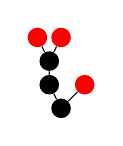
\begin{tikzpicture}[scale=.2]
\node[circle, scale=0.75, fill] (tid0) at (2.25,1.5){};
\node[circle, scale=0.75, fill] (tid1) at (1.5,3){};
\node[circle, scale=0.75, fill] (tid3) at (1.5,4.5){};
\node[circle, scale=0.75, fill, red] (tid4) at (0.75,6){};
\node[circle, scale=0.75, fill, red] (tid5) at (2.25,6){};
\draw[](tid3) -- (tid4);
\draw[](tid3) -- (tid5);
\draw[](tid1) -- (tid3);
\node[circle, scale=0.75, fill, red] (tid2) at (3.75,3){};
\draw[](tid0) -- (tid1);
\draw[](tid0) -- (tid2);
\end{tikzpicture}
\nodepart{three}
\footnotesize{4.58333}
\nodepart{four}
\footnotesize{$33\:67$}
};
 & 
\node[draw=black, rectangle split,  rectangle split parts=4] (sn0x23734a0){
\footnotesize{0.666667}
\nodepart{two}
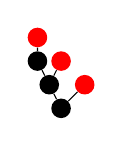
\begin{tikzpicture}[scale=.2]
\node[circle, scale=0.75, fill] (tid0) at (2.25,1.5){};
\node[circle, scale=0.75, fill] (tid1) at (1.5,3){};
\node[circle, scale=0.75, fill] (tid3) at (0.75,4.5){};
\node[circle, scale=0.75, fill, red] (tid5) at (0.75,6){};
\draw[](tid3) -- (tid5);
\node[circle, scale=0.75, fill, red] (tid4) at (2.25,4.5){};
\draw[](tid1) -- (tid3);
\draw[](tid1) -- (tid4);
\node[circle, scale=0.75, fill, red] (tid2) at (3.75,3){};
\draw[](tid0) -- (tid1);
\draw[](tid0) -- (tid2);
\end{tikzpicture}
\nodepart{three}
\footnotesize{4.34722}
\nodepart{four}
\footnotesize{$33\:33\:33$}
};
 & 
\\
};
\end{scope}
\begin{scope}[yshift=\leveltopIII cm]
\matrix (line3) [column sep=1cm] {
\node[draw=black, rectangle split,  rectangle split parts=4] (sn0x2373f60){
\footnotesize{0.111111}
\nodepart{two}
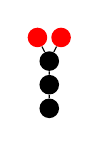
\begin{tikzpicture}[scale=.2]
\node[circle, scale=0.75, fill] (tid0) at (1.5,1.5){};
\node[circle, scale=0.75, fill] (tid1) at (1.5,3){};
\node[circle, scale=0.75, fill] (tid2) at (1.5,4.5){};
\node[circle, scale=0.75, fill, red] (tid3) at (0.75,6){};
\node[circle, scale=0.75, fill, red] (tid4) at (2.25,6){};
\draw[](tid2) -- (tid3);
\draw[](tid2) -- (tid4);
\draw[](tid1) -- (tid2);
\draw[](tid0) -- (tid1);
\end{tikzpicture}
\nodepart{three}
\footnotesize{4.5}
\nodepart{four}
\footnotesize{$1$}
};
 & 
\node[draw=black, rectangle split,  rectangle split parts=4] (sn0x2373ca0){
\footnotesize{0.444444}
\nodepart{two}
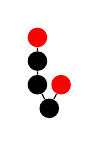
\begin{tikzpicture}[scale=.2]
\node[circle, scale=0.75, fill] (tid0) at (1.5,1.5){};
\node[circle, scale=0.75, fill] (tid1) at (0.75,3){};
\node[circle, scale=0.75, fill] (tid3) at (0.75,4.5){};
\node[circle, scale=0.75, fill, red] (tid4) at (0.75,6){};
\draw[](tid3) -- (tid4);
\draw[](tid1) -- (tid3);
\node[circle, scale=0.75, fill, red] (tid2) at (2.25,3){};
\draw[](tid0) -- (tid1);
\draw[](tid0) -- (tid2);
\end{tikzpicture}
\nodepart{three}
\footnotesize{4.125}
\nodepart{four}
\footnotesize{$50\:50$}
};
 & 
\node[draw=black, rectangle split,  rectangle split parts=4] (sn0x2374e00){
\footnotesize{0.222222}
\nodepart{two}
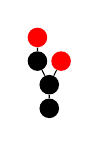
\begin{tikzpicture}[scale=.2]
\node[circle, scale=0.75, fill] (tid0) at (1.5,1.5){};
\node[circle, scale=0.75, fill] (tid1) at (1.5,3){};
\node[circle, scale=0.75, fill] (tid2) at (0.75,4.5){};
\node[circle, scale=0.75, fill, red] (tid4) at (0.75,6){};
\draw[](tid2) -- (tid4);
\node[circle, scale=0.75, fill, red] (tid3) at (2.25,4.5){};
\draw[](tid1) -- (tid2);
\draw[](tid1) -- (tid3);
\draw[](tid0) -- (tid1);
\end{tikzpicture}
\nodepart{three}
\footnotesize{4.25}
\nodepart{four}
\footnotesize{$50\:50$}
};
 & 
\node[draw=black, rectangle split,  rectangle split parts=4] (sn0x23751d0){
\footnotesize{0.222222}
\nodepart{two}
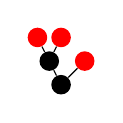
\begin{tikzpicture}[scale=.2]
\node[circle, scale=0.75, fill] (tid0) at (2.25,1.5){};
\node[circle, scale=0.75, fill] (tid1) at (1.5,3){};
\node[circle, scale=0.75, fill, red] (tid3) at (0.75,4.5){};
\node[circle, scale=0.75, fill, red] (tid4) at (2.25,4.5){};
\draw[](tid1) -- (tid3);
\draw[](tid1) -- (tid4);
\node[circle, scale=0.75, fill, red] (tid2) at (3.75,3){};
\draw[](tid0) -- (tid1);
\draw[](tid0) -- (tid2);
\end{tikzpicture}
\nodepart{three}
\footnotesize{3.66667}
\nodepart{four}
\footnotesize{$67\:33$}
};
 & 
\\
};
\end{scope}
\begin{scope}[yshift=\leveltopIIII cm]
\matrix (line4) [column sep=1cm] {
\node[draw=black, rectangle split,  rectangle split parts=4] (sn0x23740a0){
\footnotesize{0.444444}
\nodepart{two}
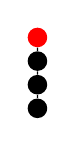
\begin{tikzpicture}[scale=.2]
\node[circle, scale=0.75, fill] (tid0) at (0.75,1.5){};
\node[circle, scale=0.75, fill] (tid1) at (0.75,3){};
\node[circle, scale=0.75, fill] (tid2) at (0.75,4.5){};
\node[circle, scale=0.75, fill, red] (tid3) at (0.75,6){};
\draw[](tid2) -- (tid3);
\draw[](tid1) -- (tid2);
\draw[](tid0) -- (tid1);
\end{tikzpicture}
\nodepart{three}
\footnotesize{4}
\nodepart{four}
\footnotesize{$1$}
};
 & 
\node[draw=black, rectangle split,  rectangle split parts=4] (sn0x2374510){
\footnotesize{0.37037}
\nodepart{two}
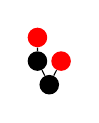
\begin{tikzpicture}[scale=.2]
\node[circle, scale=0.75, fill] (tid0) at (1.5,1.5){};
\node[circle, scale=0.75, fill] (tid1) at (0.75,3){};
\node[circle, scale=0.75, fill, red] (tid3) at (0.75,4.5){};
\draw[](tid1) -- (tid3);
\node[circle, scale=0.75, fill, red] (tid2) at (2.25,3){};
\draw[](tid0) -- (tid1);
\draw[](tid0) -- (tid2);
\end{tikzpicture}
\nodepart{three}
\footnotesize{3.25}
\nodepart{four}
\footnotesize{$50\:50$}
};
 & 
\node[draw=black, rectangle split,  rectangle split parts=4] (sn0x23757a0){
\footnotesize{0.185185}
\nodepart{two}
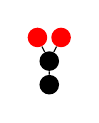
\begin{tikzpicture}[scale=.2]
\node[circle, scale=0.75, fill] (tid0) at (1.5,1.5){};
\node[circle, scale=0.75, fill] (tid1) at (1.5,3){};
\node[circle, scale=0.75, fill, red] (tid2) at (0.75,4.5){};
\node[circle, scale=0.75, fill, red] (tid3) at (2.25,4.5){};
\draw[](tid1) -- (tid2);
\draw[](tid1) -- (tid3);
\draw[](tid0) -- (tid1);
\end{tikzpicture}
\nodepart{three}
\footnotesize{3.5}
\nodepart{four}
\footnotesize{$1$}
};
 & 
\\
};
\end{scope}
\begin{scope}[yshift=\leveltopIIIII cm]
\matrix (line5) [column sep=1cm] {
\node[draw=black, rectangle split,  rectangle split parts=4] (sn0x2374200){
\footnotesize{0.814815}
\nodepart{two}
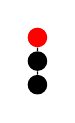
\begin{tikzpicture}[scale=.2]
\node[circle, scale=0.75, fill] (tid0) at (0.75,1.5){};
\node[circle, scale=0.75, fill] (tid1) at (0.75,3){};
\node[circle, scale=0.75, fill, red] (tid2) at (0.75,4.5){};
\draw[](tid1) -- (tid2);
\draw[](tid0) -- (tid1);
\end{tikzpicture}
\nodepart{three}
\footnotesize{3}
\nodepart{four}
\footnotesize{$1$}
};
 & 
\node[draw=black, rectangle split,  rectangle split parts=4] (sn0x23748f0){
\footnotesize{0.185185}
\nodepart{two}

\begin{tikzpicture}[scale=.2]
\node[circle, scale=0.75, fill] (tid0) at (1.5,1.5){};
\node[circle, scale=0.75, fill, red] (tid1) at (0.75,3){};
\node[circle, scale=0.75, fill, red] (tid2) at (2.25,3){};
\draw[](tid0) -- (tid1);
\draw[](tid0) -- (tid2);
\end{tikzpicture}
\nodepart{three}
\footnotesize{2.5}
\nodepart{four}
\footnotesize{$1$}
};
 & 
\\
};
\end{scope}
\begin{scope}[yshift=\leveltopIIIIII cm]
\matrix (line6) [column sep=1cm] {
\node[draw=black, rectangle split,  rectangle split parts=4] (sn0x23742d0){
\footnotesize{1}
\nodepart{two}

\begin{tikzpicture}[scale=.2]
\node[circle, scale=0.75, fill] (tid0) at (0.75,1.5){};
\node[circle, scale=0.75, fill, red] (tid1) at (0.75,3){};
\draw[](tid0) -- (tid1);
\end{tikzpicture}
\nodepart{three}
\footnotesize{2}
\nodepart{four}
\footnotesize{$1$}
};
 & 
\\
};
\end{scope}
\begin{scope}[yshift=\leveltopIIIIIII cm]
\matrix (line7) [column sep=1cm] {
\node[draw=black, rectangle split,  rectangle split parts=4] (sn0x23743a0){
\footnotesize{1}
\nodepart{two}

\begin{tikzpicture}[scale=.2]
\node[circle, scale=0.75, fill, red] (tid0) at (0.75,1.5){};
\end{tikzpicture}
\nodepart{three}
\footnotesize{1}
\nodepart{four}
\footnotesize{$$}
};
 & 
\\
};
\end{scope}
\begin{scope}[yshift=\leveltopIIIIIIII cm]
\matrix (line8) [column sep=1cm] {
\\
};
\end{scope}
\draw (sn0x2373880.south) -- (sn0x2373960.north);
\draw (sn0x2373880.south) -- (sn0x23734a0.north);
\draw (sn0x2373960.south) -- (sn0x2373f60.north);
\draw (sn0x2373960.south) -- (sn0x2373ca0.north);
\draw (sn0x23734a0.south) -- (sn0x2374e00.north);
\draw (sn0x23734a0.south) -- (sn0x2373ca0.north);
\draw (sn0x23734a0.south) -- (sn0x23751d0.north);
\draw (sn0x2373f60.south) -- (sn0x23740a0.north);
\draw (sn0x2373ca0.south) -- (sn0x23740a0.north);
\draw (sn0x2373ca0.south) -- (sn0x2374510.north);
\draw (sn0x2374e00.south) -- (sn0x23740a0.north);
\draw (sn0x2374e00.south) -- (sn0x23757a0.north);
\draw (sn0x23751d0.south) -- (sn0x23757a0.north);
\draw (sn0x23751d0.south) -- (sn0x2374510.north);
\draw (sn0x23740a0.south) -- (sn0x2374200.north);
\draw (sn0x2374510.south) -- (sn0x2374200.north);
\draw (sn0x2374510.south) -- (sn0x23748f0.north);
\draw (sn0x23757a0.south) -- (sn0x2374200.north);
\draw (sn0x2374200.south) -- (sn0x23742d0.north);
\draw (sn0x23748f0.south) -- (sn0x23742d0.north);
\draw (sn0x23742d0.south) -- (sn0x23743a0.north);
\end{tikzpicture}

%%% Local Variables:
%%% TeX-master: "thesis/thesis.tex"
%%% End: 
